%%%%%%%%%%%%%%%%%%%%%%%%%%%%%%%%%%%%%%%%%
% Wenneker Assignment
% LaTeX Template
% Version 2.0 (12/1/2019)
%
% This template originates from:
% http://www.LaTeXTemplates.com
%
% Authors:
% Vel (vel@LaTeXTemplates.com)
% Frits Wenneker
%
% License:
% CC BY-NC-SA 3.0 (http://creativecommons.org/licenses/by-nc-sa/3.0/)
% 
%%%%%%%%%%%%%%%%%%%%%%%%%%%%%%%%%%%%%%%%%

%----------------------------------------------------------------------------------------
%	PACKAGES AND OTHER DOCUMENT CONFIGURATIONS
%----------------------------------------------------------------------------------------

\documentclass[11pt]{scrartcl} % Font size
\usepackage{hyperref} % for url
\usepackage{tikz} %for RNN

%%%%%%%%%%%%%%%%%%%%%%%%%%%%%%%%%%%%%%%%%
% Wenneker Assignment
% Structure Specification File
% Version 2.0 (12/1/2019)
%
% This template originates from:
% http://www.LaTeXTemplates.com
%
% Authors:
% Vel (vel@LaTeXTemplates.com)
% Frits Wenneker
%
% License:
% CC BY-NC-SA 3.0 (http://creativecommons.org/licenses/by-nc-sa/3.0/)
% 
%%%%%%%%%%%%%%%%%%%%%%%%%%%%%%%%%%%%%%%%%

%----------------------------------------------------------------------------------------
%	PACKAGES AND OTHER DOCUMENT CONFIGURATIONS
%----------------------------------------------------------------------------------------

\usepackage{amsmath, amsfonts, amsthm} % Math packages

\usepackage{listings} % Code listings, with syntax highlighting

\usepackage[french]{babel} % English language hyphenation

\usepackage{graphicx} % Required for inserting images
\graphicspath{{Figures/}{./}} % Specifies where to look for included images (trailing slash required)

\usepackage{booktabs} % Required for better horizontal rules in tables

\numberwithin{equation}{section} % Number equations within sections (i.e. 1.1, 1.2, 2.1, 2.2 instead of 1, 2, 3, 4)
\numberwithin{figure}{section} % Number figures within sections (i.e. 1.1, 1.2, 2.1, 2.2 instead of 1, 2, 3, 4)
\numberwithin{table}{section} % Number tables within sections (i.e. 1.1, 1.2, 2.1, 2.2 instead of 1, 2, 3, 4)

\setlength\parindent{0pt} % Removes all indentation from paragraphs

\usepackage{enumitem} % Required for list customisation
\setlist{noitemsep} % No spacing between list items

%----------------------------------------------------------------------------------------
%	DOCUMENT MARGINS
%----------------------------------------------------------------------------------------

\usepackage{geometry} % Required for adjusting page dimensions and margins

\geometry{
	paper=a4paper, % Paper size, change to letterpaper for US letter size
	top=2.5cm, % Top margin
	bottom=3cm, % Bottom margin
	left=3cm, % Left margin
	right=3cm, % Right margin
	headheight=0.75cm, % Header height
	footskip=1.5cm, % Space from the bottom margin to the baseline of the footer
	headsep=0.75cm, % Space from the top margin to the baseline of the header
	%showframe, % Uncomment to show how the type block is set on the page
}

%----------------------------------------------------------------------------------------
%	FONTS
%----------------------------------------------------------------------------------------

\usepackage[utf8]{inputenc} % Required for inputting international characters
\usepackage[T1]{fontenc} % Use 8-bit encoding

\usepackage{fourier} % Use the Adobe Utopia font for the document

%----------------------------------------------------------------------------------------
%	SECTION TITLES
%----------------------------------------------------------------------------------------

\usepackage{sectsty} % Allows customising section commands

\sectionfont{\vspace{6pt}\centering\normalfont\scshape} % \section{} styling
\subsectionfont{\normalfont\bfseries} % \subsection{} styling
\subsubsectionfont{\normalfont\itshape} % \subsubsection{} styling
\paragraphfont{\normalfont\scshape} % \paragraph{} styling

%----------------------------------------------------------------------------------------
%	HEADERS AND FOOTERS
%----------------------------------------------------------------------------------------

\usepackage{scrlayer-scrpage} % Required for customising headers and footers

\ohead*{} % Right header
\ihead*{} % Left header
\chead*{} % Centre header

\ofoot*{} % Right footer
\ifoot*{} % Left footer
\cfoot*{\pagemark} % Centre footer
 % Include the file specifying the document structure and custom commands
\newtheorem{theorem}{Théorème}[section]
\newtheorem{corollary}{Corollaire}[theorem]
\newtheorem{lemma}[theorem]{Lemme}
\newtheorem{Def}[theorem]{Definition}
\newtheorem{pro}[theorem]{Proposition}

%%newcommand
\newcommand{\Xt}{\left(X_t\right)_{t\in\mathbb{Z}}}
\newcommand{\Z}{\mathbb{Z}}
\newcommand{\C}{\mathbb{C}}
\newcommand{\N}{\mathbb{N}}
\newcommand{\R}{\mathbb{R}}
\newcommand{\var}[1]{\mathbb{V}\left(#1\right)}
\newcommand{\E}[1]{\mathbb{E}\left(#1\right)}
\newcommand{\bb}[1]{\mathcal{BB}\left(0,#1\right)}
\newcommand{\bbn}[1]{\mathcal{BBN}\left(0,#1\right)}
%----------------------------------------------------------------------------------------
%	TITLE SECTION
%----------------------------------------------------------------------------------------

\title{	
	\normalfont\normalsize
	\textsc{CNAM}\\ % Your university, school and/or department name(s)
	\vspace{25pt} % Whitespace
	\rule{\linewidth}{0.5pt}\\ % Thin top horizontal rule
	\vspace{20pt} % Whitespace
	{\huge Series temporelles : ARIMA, LSTM?}\\ % The assignment title
	\vspace{12pt} % Whitespace
	\rule{\linewidth}{2pt}\\ % Thick bottom horizontal rule
	\vspace{12pt} % Whitespace
}

\author{\LARGE Jérôme Petit} % Your name

\date{\normalsize\today} % Today's date (\today) or a custom date

\begin{document}

\maketitle % Print the title

%----------------------------------------------------------------------------------------
%	FIGURE EXAMPLE
%----------------------------------------------------------------------------------------
%
\section{Introduction}


\section{Séries temporelles}
Une série temporelle ou série chronologique est une suite d'observations d’un phénomène faites au cours du temps. Cette notion s'étend à de nombreux domaines, tout relevé de données, de flux ou d'information est une série temporelle : indice boursier, population française, trafic Internet, etc. Ses données réelles obtenues sont des suites finies indexés par un temps continu ou discret. Les modèles mathématiques utilisées pour modélisées ses séries temporelles sont eux de dimension infinie.


Dans la suite de ce document, on notera l'observation $x_t$ pour tout $t=1,...,T$ d'une variable aléatoire $X_t(\omega)$. Si le processus a été spécifié, estimé et validé, on peut alors l'utiliser pour effectuer une prévision. On notera alors $\hat{X}_T(h)$ le prédicteur de la variable aléatoire $X_{T+h}$. Ce prédicteur permettra de calculer la prévision $\hat{x}_T(h)$ comme étant la réalisation de $\hat{X}_T(h)$. 


Afin d'étudier les séries temporelles, nous allons utiliser les moments d'ordre 1 et 2. Le moment d'ordre 1 permet de déterminer la tendance d'un processus et le moment d'ordre 2 permet de déterminer la variance du processus et d'étudier la dépendance temporelle du processus.
\begin{Def}\label{defMom}
Soit un processus $\Xt$ un processus du second ordre (i.e. $\E{X_t^2}<\infty$).
\begin{itemize}
\item[i)]La fonction moyenne $m$ du processus $\Xt$ est l'espérance non conditionnelle du processus~:~$m(t)=\E{X_t}$, $\forall t\in \Z$.
\item[ii)]La fonction d'autocovaraince de retard $k$, notée $\gamma(k)$, du processus $\Xt$ est définie de la manière suivante, $\forall t, k\in\Z$~:
$$
\gamma(k)=cov\left(X_t,X_{t+k}\right)=\E{\left(X_t-\E{X_t}\right)\left(X_{t+k}-\E{X_{t+k}}\right)}
$$
\item[iii)]La fonction d'autocorrélation de retard $k$ (ACF), notée $\rho(k)$, du processus $\Xt$ est définie de la manière suivante, $\forall t, k\in\Z$~:
$$
\rho(k)=\frac{\gamma(k)}{\sigma_{X_t}\sigma_{X_{t+k}}}
$$
avec $\sigma_{X_t}$ l'écart type du processus au temps $t$~:~$\sigma_{X_t}=\sqrt{\gamma(0)}$
\item[iv)]La fonction d'autocorrélation partielle de retard $k$ (PACF), notée $r(k)$, du processus $\Xt$ est définie de la manière suivante, $\forall t, k\in\Z$~:
$$
r(k)=\frac{cov(X_t-X_t^*,X_{t+k}-X_{t+k}^*)}{\sqrt{var(X_t-X_t^*)}\sqrt{var(X_{t+k}-X_{t+k}^*)}}
$$
avec $X_t^*$ la régression affine de $X_t$ sur $X_{t+1},X_{t+2},..., X_{t+k-1}$ et $X^*_{t+k}$ est la régression affine de $X_{t+k}$ sur $X_{t+k-1},X_{t+k-2},...,X_{t+1}$.
\end{itemize}
\end{Def}
On dit que le processus est centré si pour tout t $m(t)=0$. Le coefficient $r(k)$ mesure la liaison entre les variables $X_t$ et $X_{t+k}$ une fois que l'on a retranché l'influence des variables intermédiaires. On peut exprimer le terme d'autocorellation partielle à l'aide d'un régression linéaire.
\begin{pro}
Le coefficient $r(k)$ définit dans (\ref{defMom}) est le coefficient de $X_t$ dans la régression linéaire de $X_{t+k}$ sur 1, $X_t$, $X_{t+1}$,..., $X_{t+k-1}$.
\end{pro}

La définition de l'autocorelation partielle peut s'écrire à l'aide de l'auto correlation~:
$$
\left(
\begin{tabular}{c}
$c_1$\\
$c_2$\\
. \\
. \\
r(k)
\end{tabular}
\right) = 
\left(
\begin{tabular}{cccc}
1 & $\rho(1)$ & . & $\rho(k-1)$\\
$\rho(1)$ & 1 & . & $\rho(k-2)$\\
. & . & . & . \\
. & . & . & . \\
$\rho(k-1)$ & $\rho(k-2)$ & . & 1
\end{tabular}
\right)^{-1}
\left(
\begin{tabular}{c}
$\rho(1)$\\
$\rho(2)$\\
. \\
. \\
$\rho(k)$
\end{tabular}
\right)
$$



Dans la pratique, on aura un échantillon fini, il faudra donc estimer ses moments à partir de l'échantillon fourni. Dans la suite on appellera ses estimations des \textit{moments empiriques}~:
\begin{align*}
\overline{X}_T &= \frac{1}{T}\sum_{t=1}^TX_t\\
\overline{\gamma}(h)&=\frac{1}{T-h}\sum_{t=h+1}^T(X_t-\overline{X})(X_{t-h}-\overline{X}), 0\leq h\leq T-1\\
\overline{\rho}(h)&=\frac{T}{T-h}\frac{\sum_{t=h+1}^T(y_t-\overline{y})(y_{t-h}-\overline{y})}{\sum_{t=1}^T(y_t-\overline{y})^2}, 0\leq h\leq T-1,\\
\end{align*}
en remplaçant $T-h$ par $T$ dans le calcul de l'autocorrélation (resp. d'autocovariance), on obtient un estimateur avec biais. On remarque que lorsque h est proche du nombre de termes dans l'échantillon alors le calcul de l'autocorrélation (resp. autocovariance) empirique est de faible qualité car elle dépend de peu de terme de la série temporelle.

\subsection{Processus à mémoire}
L'ACF permet de mesurer la persistence (ou la mémoire) d'un processus, elle va pouvoir classer les processus en fonction de leur mémoire. On va considérer les processus sans mémoire, à mémoire courte et à mémoire longue.


Un \textit{processus sans mémoire} est un processus tel que pour tout $t\in\Z$ $X_t$ n'est pas corrélé à $X_{t-1}, X_{t-2},...$. Les bruits blancs sont des processus sans mémoire.


\begin{Def}\label{BB}
Un bruit blanc $\epsilon_t$ est une suite de variable aléatoire non corrélées, mais pas nécessairement indépendantes de moyenne nulle et de variance constante $\sigma^2$. On note $\epsilon_t\sim \bb{\sigma^2}$.
\newline 
Un \textit{bruit blanc fort} est un bruit blanc dont les variables aléatoires sont indépendantes.
\end{Def}
Pour un bruit blanc $X_t$, on a~:
\begin{itemize}
\item $\E{X_t}=0$
\item $\gamma(h)=0$ si $h\not =0$
\end{itemize}
De la même manière on définit~:
\begin{Def}\label{BBG}
Un bruit blanc gaussien $\epsilon_t$ est une suite de variable aléatoire i.i.d de loi normale $\mathcal{N}\left(0,\sigma^2\right)$. On note $\epsilon\sim \bbn{\sigma^2}$
\end{Def}
Un bruit blanc gaussien est également un processus sans mémoire.


La dénomination de \textit{bruit} vient du fait que ce processus ne contient aucune information d'autocorrélation. Ainsi aucun signal déterministe ne peut être extrait de ce processus. 


Il existe également des processus dont l'ACF est géométriquement bornée et décroit rapidement vers 0, on parle alors de processus à mémoire courte. C'est le cas des processus de type ARMA, AR ou MA.
\begin{Def}\label{defCourte}
Un processus est dit à mémoire courte s'il possède une ACF, $\rho(k)$, telle que~:
$$
\rho(k)\leq Cr^{k}
$$
avec $C>0$ et $0<r<1$
\end{Def}
Par exemple, les modèles MA(1) et AR(1) sont des processus à mémoire courte. En effet, pour un processus $X_t$ qui est un processus MA(1), on a~:~$X_t=\epsilon_t+\theta\epsilon_{t-1}$ avec $\epsilon_t$ un bruit blanc de variance $\sigma^2$, on a~:
\begin{align*}
\E{X_t}&=0\\
\gamma(0)&=\sigma^2(1+\theta^2)\\
\gamma(1) &= \theta\sigma^2\\
\gamma(h)&= 0, \forall h\not=0,1,-1
\end{align*}
ainsi $\rho(h)=0$ pour tout $h>1$.
\begin{Def}
Un processus est dit à mémoire longue s'il possède une ACF, $\rho(k)$ qui a le comportement asymptotique suivant~:
$$
\rho(k)\sim_{k\rightarrow \infty} Ck^{-\alpha}
$$
avec $C>0$ une constante et $\alpha\in ]0,1[$.
\end{Def}
Pour des processus à mémoire longue la série des autocorellations est absolument divergente. Les processus fractionnaires de type ARFIMA permettent de reproduire ce comportement.

\subsection{Stationnarités}
\subsubsection{Stationnarités faibles et fortes}
\begin{Def}\label{staForte}
Stationnarité stricte ou forte~:~$\left(X_t\right)_{t\in\mathbb{Z}}$ est un processus stationnaire au sens strict si~:~$\forall n\in \mathbb{N}, \forall (t_1,...,t_n), \forall h\in\mathbb{Z}$ la loi de $(X_{t_1},...,X_{t_n})$ est identique à la loi de $(X_{t_1+h},...,X_{t_n+h})$
\end{Def}
D'après le théorème de Kolmogorov, on en déduit qu'un processus $\left(X_t\right)$ est stationnaire au sens fort si et seulement si la loi de $X_t$ est identique à la loi de $X_{t+h}$ quelque soit $h$. Cette condition de stationnarité est très contraignante et relativement peu observée en pratique. On remarque que pour un processus stationnaire strict $X_t$ admettant des moments d'ordre 1 et 2 finis, on a~:
$$
\mathbb{E}\left(X_t\right)=\mathbb{E}\left(X_{t+h}\right), \forall h\in \mathbb{N}
$$
on pose~:~$\mathbb{E}\left(X_t\right)=\mathbb{E}\left(X_0\right)=\mu$. Pour la covariance, on a~:
\begin{align*}
Cov\left(X_t,X_{t+h}\right)& = \mathbb{E}\left((X_t-\mu)(X_{t+h}-\mu)\right)\\
&= \mathbb{E}\left((X_0-\mu)(X_{h}-\mu)\right)
\end{align*}
la dernière égalité vient du fait que $(X_t,X_{t+h})$ a la même distribution que $(X_0,X_h)$.
On remarque donc que les processus stationnaire strict ont des moments d'ordre 1 et 2 indépendant du temps $t$. C'est cette notion qui va être utilisée pour des définir les processus stationnaires au sens faible.
\begin{Def}\label{staFaible}
Stationnarité faible ou du second ordre~:~
$\left(X_t\right)_{t\in\mathbb{Z}}$ est un processus stationnaire du second ordre (ou processus faiblement stationnaire ) s'il vérifie~:
\begin{itemize}
\item[i)]$\forall t\in\mathbb{Z},~\mathbb{E}\left(X_t\right)=m $ 
\item[ii)]$\forall t\in\mathbb{Z},~\mathbb{V}\left(X_t\right)=\sigma^2 $ 
\item[iii)]$\forall t,h\in\mathbb{Z},~Cov\left(X_t,X_{t+h}\right)=Cov\left(X_0,X_h\right)=\gamma\left(h\right) $ 
\end{itemize}
On note $\gamma(h)$ l'autocovariance d'ordre $h$ de $X_t$ .
\end{Def} 
Un processus fortement stationnaire est un processus stationnaire du second ordre. L'inverse n'est pas généralement vrai. Dans la suite les processus stationnaires désigneront les processus stationnaires du second ordre.


On peut généraliser la définition de processus stationnaire à l'ordre deux aux cas vectoriel~:
\begin{Def}\label{staFaibleVec}
Stationnarité vectorielle faible ou du second ordre~:~
$\left(X_t\right)_{t\in\mathbb{Z}}$ est un processus stationnaire vectoriel (n,1) du second ordre (ou processus faiblement stationnaire ) s'il vérifie~:
\begin{itemize}
\item[i)]$\forall t\in\mathbb{Z},~\mathbb{E}\left(X_t\right)=m $ 
\item[ii)]$\forall t,h\in\mathbb{Z},~\E{(X_t-m)(X_{t+h}-m)}=\gamma\left(h\right) $ est indépendant de $t$ 
\end{itemize}
\end{Def} 
Ainsi pour tout $h$ la matrice $\gamma(h)$ est une matrice carrée de taille n indépendante de t.

 

Sous certaine condition sur les coefficients, les processus stationnaires sont stables par combinaison linaires : 
\begin{pro}
Si $\Xt$ est un processus stationnaire et $(a_i)_{i\in \mathbb{Z}}$ est une suite de réels absolument convergente alors le processus : 
$$
Y_t=\sum_{i\in\mathbb{Z}}a_i X_{t-i}
$$
est un processus stationnaire
\end{pro}
Une conséquence de cette proposition est que la différence ou la moyenne de processus stationnaire est un processus stationnaire.



Pour un processus stationnaire, la fonction d'auto-correlation partielle satisfait la relation~:
$$
r(k) = \frac{\left|P_k^*\right|}{\left|P_k\right|}
$$
avec~:
$$
P_k=\left(\begin{tabular}{cccc}
1 & $\rho(1)$ & . & $\rho(k-1)$\\
$\rho(1)$ & 1 & . & $\rho(k-2)$\\
. & . & . & .\\
$\rho(k-1)$ & $\rho(k-2)$ & . & 1
\end{tabular}
\right)
$$
et 
$$
P_k^*=\left(\begin{tabular}{cccc}
1 & $\rho(1)$ & . & $\rho(1)$\\
$\rho(1)$ & 1 & . & $\rho(k-2)$\\
. & . & . & .\\
$\rho(k-1)$ & $\rho(k-2)$ & . & 1\\
\end{tabular}
\right)
$$
Les 3 premières autocorrélations partielles sont donc déterminées par les relation suivantes~:
\begin{align*}
r(1)&=\rho(1)\\
r(2)&= \frac{\rho(2)-\rho(1)^2}{1-\rho(1)^2}\\
r(3)&=\frac{\rho(1)^3-\rho(1)\rho(2)(2-\rho(2))+\rho(3)(1-\rho(1)^2)}{1-\rho(2)^2-2\rho(1)^2(1-\rho(2))}
\end{align*}
On peut estimer l'auto corrélation partielle par une méthodes des moindres carrées~:
$$
x_{t+1} = \hat{c} + \hat{r}(1)x_{t-1}+\hat{r}(2)x_{t-2}+...+\hat{r}(k)x_{t-k+1}\,,\forall k \in \Z
$$
A l'aide de la relation précédente $\hat{r}(k)=\frac{\left|P_k^*\right|}{\left| P_k \right|}$, l'estimation de $\hat{r}(k)$ permet d'obtenir les estimations de $\hat{\rho}$.



La stationnarité d'un processus permet d'estimer les moments non conditionnels de $X_{T+h}$ en utilisant les moments empiriques. Ainsi on peut utiliser comme prédicateur naturel de $X_{T+h}$ un estimateur de l'espérance non conditionnelle $\E{X_{T+h}}$ en particulier la moyenne empirique, i.e.~:~$\hat{X}_{T+h}=\frac{1}{T}\sum_{t=1}^TX_t$. Mais on se rend compte que cette prévision est extrêmement grossière car pour n'importe quel horizon $h>0$, le prédicateur est identique, illustrant ainsi que la dynamique du processus n'est pas prise en compte dans ce type de prédicateur.

\subsubsection{localement stationnaire}
Dahlaus a défini dans \cite{locally} la notion de stationnarité locale pour les processus linéaires. Afin de la définir, j'introduit quelques notions nécessaires. La notion de localement stationnaire est utilisée pour des processus dont la représentation dépend du temps. Cela signifie, par example qu'un processus AR(1) dépendant du temps s'écrit : $X_t+\alpha_tX_{t-1}=\epsilon_t$, les coefficients du modèle dépendent du temps. On ne peut plus avoir de stationnarité globale car la valeur de se coefficient va changer selon $t$. De plus son estimation va dépendre de $t$ et de la taille de l'échantillon $T$ à l'instant $t$. Le paramètres du modèle sont calculés sur l'échantillon $[1,T]$ pour chaque instant $t$, afin d'éviter les problèmes d'estimation sur une taille finie et de passage à la lime quand $t\rightarrow \infty$, on réalise un changement d'échelle $\frac{t}{T}$ afin d'estimer les paramètres sur l'intervalle $[0,1]$ et le passage à la limite se fera quand $t\rightarrow 1$. Dans \cite{locally}, la définition est donnée pour des processus linéaire (MA($\infty$)). Rappelons que la représentation d'un processus linéaire $X_{t,T}$ est~:
$$
X_{t,T}=\mu\left(\frac{t}{T}\right)+\sum_{j=-\infty}^\infty a_{t,T}(j)\epsilon_{t-j}
$$
L'approximation de se processus va reposer sur l'estimation de $a_{t,T}(j)\approx a(\frac{t}{T},j)$ et donc imposer certaine régularité sur le coefficient a. 


L'idée principale de la stationnarité locale est que pour tout $u_0\in [0,1]$ le processus $X_{t,T}$ peut être approché par un processus stationnaire $\tilde{X}_t(u_0)$. Le processus stationnaire $\tilde{X}_t(u_0)$ s'écrit~:
$$
\tilde{X}_t(u)=\mu(u)+\sum_{j=-\infty}^\infty a(u,j)\epsilon_{t-j}
$$

\subsubsection{Non stationnarité}
La stationnarité d'ordre 2 se définie comme une invariance des moments d'ordre 1 et 2. Par opposition, on dira qu'une série est non-stationnaire si elle n'est pas stationnaire. La classe des processus non stationnaire est plus vaste que celle des processus stationnaire. Parmi les processus non stationnaire Nelson et Plosser \cite{NonSta} ont retenu deux classes de processus non-stationnaires : les processus TS \textit{(trend stationary)} et les processus DS \textit{(difference stationary)}. Les premiers correspondent à une non-stationnarité de type déterministe alors que les seconds correspondent à une non-stationnarité de type stochastique.
\begin{Def}
$\Xt$ est un processus non-stationnaire TS s'il peut s'écrire sous la forme $X_t = f(t)+Z_t$ où $f(t)$ est une fonction déterministe du temps et $Z_t$ est un processus stationnaire.
\end{Def}
L'exemple le plus simple est celui de la tendance linéaire bruitée~:~$X_t=a+bt+\epsilon_t$. Ce processus admet une tendance déterministe $a+bt$. Les processus non-stationnaire TS non pas de persistance des chocs. L'influence d'un choc subit à un instant $\tau$ aura tendance à s'estomper au cours du temps. La variable rejoint alors sa dynamique à long terme déterminée par $f(t)$. Cette propriété est une conséquence directe de la décomposition de Wold (\ref{Wold}).
\begin{Def}
Un processus $\Xt$ est un processus non-stationnaire DS ou intégré d'ordre $d$ si le processus obtenu après $d$ différenciation est stationnaire.
\end{Def}
Les processus ARIMA sont des processus non-stationnaires DS car par différenciation un processus ARIMA se ramène à un processus stationnaire ARMA.


\subsection{Prédiction de séries temporelles}
La prédiction des séries temporelles consiste à construire à partir des données $X_t$ avec $0\leq t\leq T$ une série $\hat{X}_T(h)$ tel que pour tout $h$  $\hat{X}_T(h)$ approxime $X_{T+h}$. 


Les propriétés qui caractérisent un bon estimateur sont le fait d'être sans biais et de variance minimale. Afin d'étudier ses propriété on définit la variable d'erreur de prévision à l'horizon h~:
$$
e_{T+h} = X_{T+h}-\hat{X}_T(h)
$$
La caractéristique principale d'un bon prédicteur est de minimiser cette erreur de prévision selon une certaine métrique. Les métriques standards sont~:~l'erreur moyenne \textit{ME}, l'erreur absolue moyenne \textit{MAE}, l'erreur quadratique moyenne \textit{MSE}~:
\begin{align*}
ME&=E\left(e_{T+h}\right)\\
MAE&=E\left(\left|e_{T+h}\right|\right)\\
MSE&=E\left(e_{T+h}^2\right)
\end{align*}
Un prédicteur couramment utilisé est le processus linéaire. 
\begin{Def}
Un processus $\Xt$ est un processus linéaire s'il admet une décomposition de la forme suivante, $\forall t \in \Z$~:
$$
X_t = \sum_{i=-\infty}^{\infty}a_i\epsilon_{t-i}\,,
$$
où $\epsilon_t$ est un bruit blanc fort et $a_i$ est absolument sommable.
\end{Def}
L'utilisation des processus linéaire vient du Théorème de Wold, qui montre que tout processus stationnaire à l'ordre 2 peut s'écrire sous la forme d'un processus linéaire
\begin{theorem}\label{Wold}
Soit $X_t$ un processus stationnaire alors il existe une bruit blanc au sens faible $\epsilon_t$ et des coefficients réels $\left(\Psi_t\right)$ tel que~:
$$
X_t = m+\sum_{j\geq 0}\Psi_j\epsilon_{t-j}
$$
avec $m$ le moment d'ordre 1 de $X_t$
\end{theorem}
En utilisant le théorème de Wold, on sait qu'un processus stationnaire $X_t$ est aussi un processus linéaire. Ainsi sur un échantillon de taille $T$, on connait le meilleur prédicateur $\hat{X}_T(h)$ au sens de la plus faible erreur quadratique moyenne. On note $I_T$ la sigma algèbre engendrée par $X_1,...,X_T$ et $M_T$ le sous espace vectoriel engendré par les variables $X_1,...,X_T$ muni de la norme $L^2$. Il s'agit du prédicteur des moindres carrées~:
$$
\hat{X}_T(h)=E\left(X_{T+h}|I_T\right)=argmin_{Y\in M_T}\left(||X_{T+h}-Y||^2\right)
$$
Dans le cas des processus linéaire, l'erreur de prévision est d'espérance nulle~:
$$
E(e_{T+h}) = E(X_{T+h})-m-\sum_{i= 0}^{h-1}\Psi_iE(\epsilon_{T+h-i})=0
$$
et de variance~:
$$
V(e_{T+h}) = \sigma^2\sum_{i=0}^{h-1}\Psi_i^2
$$
La variance de l'erreur permet de déterminer l'intervalle de confiance. Ainsi pour un processus gaussien, on obtient un intervalle de confiance~:
$$
\hat{X}_T(h)\pm t_{1-\alpha}\sigma\sqrt{\sum_{i=0}^{h-1}\Psi_i^2}
$$
avec $t_{1-\alpha}$ le quantile d'ordre $1-\alpha$. Ces résultats sur la qualité de l'estimateur sont valable dans le cas où l'on connait les coefficient de l'estimateur ce qui en pratique n'arrive pas. Donc la qualité de la prédiction des coefficients va impacter la qualité de la prédiction et ajouter de l'incertitude.


Dans l'intevalle de confiance la variance de l'erreur est constante au cours du temps, mais ce n'est pas le cas pour des processus de type GARCH par example dans ces cas là, il est intéressant d'étudier la variance conditionnelle et l'espérance conditionnelle.
\subsection{Horizon de prévision}
Dans le cas de processus stationnaire, la loi de distribution conditionnelle converge vers la loi de distribution non conditionnelle lorsque l'horizon tend vers l'infini, i.e~: $L(X_{T+h}|I_T)\rightarrow L(X_0)$. Seule la vitesse de convergence diffère en fonction de la mémoire du processus. Plus la mémoire du processus est courte et plus la vitesse de convergence est grande et inversement.
Ainsi lorsqu'on utilise en prévision un processus ARMA, il est particulièrement recommandé que l'horizon soit de très court terme (h=1 ou 2) car ce type de processus étant à mémoire courte, au bout de quelques pas le prédicteur va être égal à la moyenne non conditionnelle de la série et l'on ne peut pas faire de prédiction à long terme. Si l'on désire effectuer des prévisions à long terme les processus à mémoire longue sont plus intéressants. 

\subsection*{Exemple}
Soit $X_t$ un processus AR(1) stationnaire~:
$$
X_t = \phi X_{t-1}+\epsilon_t
$$
avec $|\phi|<1$, le prédicteur d'horizon h=1 s'écrit~:
$$
\hat{X}_t(1)=E(X_{t+1}|X_t,...,X_1)=\phi X_t
$$
et donc pour $h>0$, on a~:
$$
\hat{X}_t(h)=E(X_{t+h}|X_t,...,X_1)=\phi^hX_t
$$
ainsi le prédicteur $\hat{X}_t(h)$ converge vers l'espérance de $X_t$ quand $h\rightarrow \infty$ . La vitesse de convergence est inversement proportionnelle à la valeur du paramètre $\phi$. 



Les moments empiriques convergent vers les moments théoriques. Mais malgré cette convergence, l'autocovariance empirique fournit un estimateur très pauvre de $\gamma(h)$ pour des valeurs h proche de la taille de l'échantillon. A titre indicatif, Box et Jenkins recommandent de n'utiliser ces quantités que si $T>50$ et $h<T/4$.
Lorsque l'on estime les modèles, on calcule des autocavariances empiriques et l'on doit donc s'assurer que ces autocovariances sont significativement non nulles. Pour cela on utilise le résultat suivant~:
\begin{pro}
Si $\Xt$ est un processus linéaire tel que~:
$$
X_t = \sum_{j\in \mathbb{Z}}\phi_j\epsilon_{t-j},
$$
avec $\epsilon_t$ une suite de variable i.i.d centrée tel que $\mathbb{E}\left(\epsilon_t^4\right) = \eta\mathbb{E}\left(\epsilon_t^2\right)^2<+\infty$,* $\mathbb{E}\left(\epsilon_t^2\right)=\sigma^2$ et avec $\phi_j$ une série réelle absolument convergente. Alors l'autocovariance enmpirique converge en loi vers l'autocovariance :
$$
\left(\begin{array}{c}
\overline{\gamma}_T(0)\\
.\\
.\\
.\\
\overline{\gamma}_T(p)\\
\end{array}\right)\rightarrow
 \mathcal{N}\left(
\left(\begin{array}{c}
\gamma(0)\\
.\\
.\\
.\\
\gamma(p)\\
\end{array}\right),V\right)\,,
$$
avec $V$ la matrice de variance covariance~:
$$
V=\left[\eta\gamma(h)\gamma(k)+\sum_{i\in\mathbb{Z}}\gamma(i)\gamma(i+k-h)+\gamma(i+k)\gamma(i-h)\right]_{h,k=0,...,p}
$$
\end{pro}
\section{Processus}
\subsection{Processus MA}
\begin{Def}
Le processus $\Xt$ est une moyenne mobile d'ordre q s'il existe un bruit blanc $\epsilon_t\sim BB(0,\sigma^2)$ et des réels $\theta_1,...,\theta_q$ tels que~:~
$$
X_t=m+\epsilon_t+\theta_1\epsilon_{t-1}+...+\theta_q\epsilon_{t-q}
$$ 
On note MA(q) une moyenne mobile d'ordre q.
\end{Def}
Un processus MA(q) est stationnaire, la fonction d'autocovariance est ~:
$$
\gamma(h)=\left\{\begin{array}{cc}
0 & \textrm{si |h|>q}\\
\sigma^2\left(1+\sum_{i=1}^q\theta^2_i\right) & h=0\\
\sigma^2 \theta^2_q & h=q\\
\sigma^2\left(\theta_h+\sum_{i=h+1}^q\theta_i\theta_{i-h}\right) & \textrm{si }0<h<q\\
\end{array}
\right.
$$
Il en résulte que la fonction d'autocorrélation s'écrit~:
$$
\gamma(h)=\left\{\begin{array}{cc}
0 & \textrm{si |h|>q}\\
1 & h=0\\
\frac{\theta_h+\sum_{i=h+1}^q\theta_i\theta_{i-h}}{1+\theta_1^2+...+\theta_q^2} & \textrm{si } 0<h\leq q\\
\end{array}
\right.
$$
Il n'y a pas de résultats particulier pour les autocorrélations partielles.
\subsubsection{Processus multidimensionnel : VMA(q)}
\begin{Def}
Un processus vectoriel $\Xt$ de dimension (n,1) admet une représentation VMA d'ordre q, notée VMA(q) si~:
$$
X_t = \mu + \epsilon_t +\Psi_1\epsilon_{t-1}+\Psi_2\epsilon_{t-2}+...+ \Psi_q\epsilon_{t-q}
$$
ou de façon équivalent~:
$$
X_t = \mu+\Psi(L)\epsilon_t
$$
où $\mu$ désigne l'espérance du processus vectoriel, $\Psi(L)=\sum_i\Psi_iL^i$ avec $\Psi_0=1$. Le vecteur des innovations $\epsilon_t$ est i.i.d. centrée et de matrice covariance définie positive.
\end{Def}


Le théorème de Wold (\ref{Wold}) s'applique également dans le cas multidimensionnel. En effet si un processus vectoriel est stationnaire à l'ordre 2 alors on peut le représenter sous la forme d'un processus VMA($\infty$).
\subsection{Processus AR}
\begin{Def}
Un processus $\Xt$ est un processus auto-régressif d'ordre p noté AR(p) si~:
\begin{itemize}
\item[i)] $\Xt$ est stationnaire
\item[ii)] $\Xt$ vérifie~:
$$
X_t = \mu + \phi_1X_{t-1}+...+\phi_pX_{t-p}+\epsilon_t
$$
avec $\phi_p\not=0$ et $\epsilon_t\sim BB(0,\sigma^2)$
\end{itemize}
\end{Def}
On pose $\Phi(z)=1-\phi_1z-...-\phi_pz^p$, un processus AR(p) peut s'écrire à l'aide de polynôme de retard~:
$$
\Phi(L)X_t = \mu + \epsilon_t
$$
A l'aide de cette formulation, on en déduit les racines du polynôme $\Phi$ sont toutes de module strictement supérieur à 1.
\begin{pro}
Soit $\Xt$ un processus AR(p), alors~:
\begin{itemize}
\item $\mathbb{E}\left(X_t\right) = \frac{\mu}{1-\phi_1-...-\phi_p}$\\
\item on pose $Y_t=X_t-\mathbb{E}\left(X_t\right)$ alors $Y_t$ est un processus AR(p) d'espérance nulle
\end{itemize}
\end{pro}
Les processus AR(p) sont des processus stationnaires, on a vu que les racines du polynômes de retard sont toutes strictement supérieure à 1, cela signifie que l'on peut inverser le polynôme de retard. Ainsi tout processus AR(p) peut s'écrire : $X_t = \Phi(L)^{-1}\left(\mu + \epsilon_t\right)$. L'inverse donnant une somme infinie, cela veut dire que tout processus AR(p) peut s'écrire sous la forme MA($\infty$).

\subsubsection{Propriétés des processus AR(p)}
On a vu précédemment que d'un processus AR(p) admettant une espérance non nulle, on pouvait toujours se ramenait à un processus AR(p) d'espérance nulle. Dans la suite on considérera le processus AR(p) d'espérance nulle. L'autocovariance s'écrit pour tout h>0 : 
\begin{align*}
\gamma(h)&= Cov(X_t,X_{t-h})\\
&= \mathbb{E}\left(X_tX_{t-h}\right)\\
&= \sum_{i=1}^p\phi_i\mathbb{E}\left(X_{t-i}X_{t-h}\right)+\mathbb{E}\left(\epsilon_tX_{t-h}\right)\\
&= \sum_{i=1}^p\phi_i\gamma(h-i)
\end{align*}

Pour h=0, on a~:
\begin{align*}
\gamma(0)&= \mathbb{E}\left(X_t^2\right)\\
&= \sum_{i=1}^p\phi_i\mathbb{E}\left(X_{t-i}X_{t}\right)+\mathbb{E}\left(\epsilon_tX_{t}\right)\\
&= \sum_{i=1}^p\phi_i\gamma(i)+\mathbb{E}\left(\epsilon_t\epsilon_{t}\right)\\
&=\sum_{i=1}^p\phi_i\gamma(i)+\sigma^2
\end{align*}
On a de même pour l'autocorrélation~:~$\rho(h)=\phi_1\rho(h-1)+...+\phi_p\rho(h-p)$ pour tout h>0.
Ces équations sont appelés equation de Yule-Walker. 
On a une relation de récurrence~:
$$
\rho(0)=1=\sum_{i=1}^p\phi_i\rho(i)+\frac{\sigma^2}{\gamma(0)}
$$
d'où~:
$$
\gamma(0)=\frac{\sigma^2}{1-\sum_{i=1}^p\phi_i\rho(i)}
$$
Les equations de Yule-Walker peuvent s'écrire~:
$$
\left(
\begin{array}{cccc}
1 & \rho(1) & ... & \rho(p-1)\\
\rho(1) & 1 & ... &  \rho(p-2)\\
\rho(2) & \rho(1) & ... & \rho(p-3)\\
.. & ... & ... & ...\\
\rho(p-1) & \rho(p-1) & ... & 1
\end{array}
\right)
\left(
\begin{array}{c}
\phi_1\\
. \\
. \\
.\\
\phi_p
\end{array}
\right)=\left(
\begin{array}{c}
\rho(1)\\
. \\
. \\
.\\
\rho(p)
\end{array}
\right)
$$
Les solutions de ce système sont données par les valeurs initiales $\rho(i)$. Ainsi si l'on peut estimer les corrélation sur un échantillon donné on pourra en déduire les coefficients du processus AR(p).


Une autre propriété intéressante pour les processus AR(p) est la valeur des ACF et PACF, ce qui permettra de déterminer $p$ lors de l'estimation des processus.
\begin{pro}
Soit $\Xt$ un processus AR(p) alors~:
\begin{itemize}
\item[i)] $|\rho(h)|$ et $\gamma(h)$ décroissent exponentiellement avec h\\
\item[ii)] l'auto corrélation partielle est nulle pour h>p
\end{itemize}
\end{pro}
On peut utiliser le polynome de retard afin de déterminer l'autocorrelation des processus AR.
\begin{pro}
Si le polynome de retard $\Phi(L)$ définissant le processus AR(p) (i.e. $\Phi(L)X_t=m+\epsilon_t$ admet $p$ racines distinctes $(\lambda_i)^p_{i=1}$, l'autocorellation d'ordre k est déterminée par la relation~:
$$
\rho_k = A_1\left(\frac{1}{\lambda_1}\right)^k+...+A_p\left(\frac{1}{\lambda_p}\right)^k\,,
$$
où les paramètres $A_i$ sont des constantes déterminées par les conditions initiales.
\end{pro}
Il en résulte que si les racines du  polynome de retard sont de modules strictement supérieur à 1 alors l'autocorrélation tend vers zéro. Si les racines sont réels on a une exponentielle amortie et si les racines sont complexes on aura une sinusoïdale amortie.
\subsubsection*{Exemples}
Contrairement aux processus MA(q) les processus AR(p) ne sont pas forcement des processus stationnaires. Cela va dépendre des valeurs des racines du polynome de retard définissant le processus.  Par exemple, ci dessous on a défini un processus AR(4), graphiquement on voit que la processus semble être stationnaire.  On a le comportement attendu au niveau des coefficients ACF et PACF.
\begin{figure}[h]
   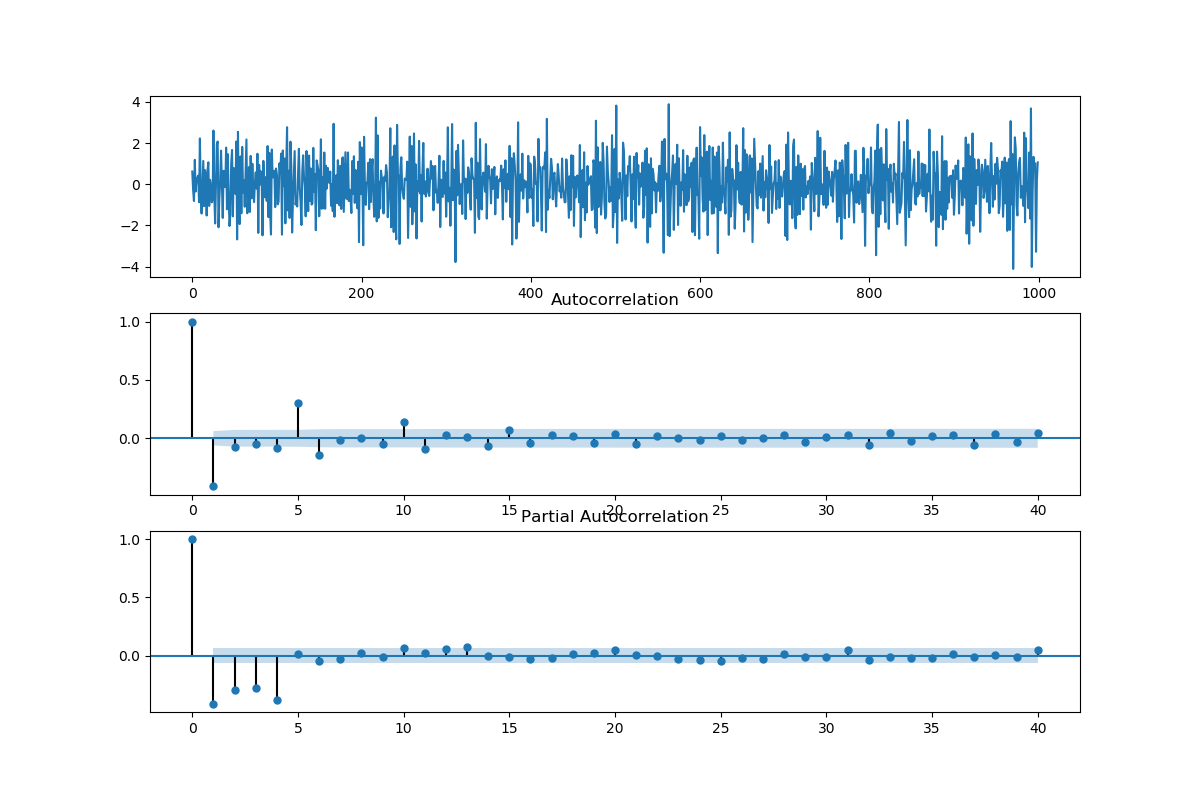
\includegraphics[scale=.5]{AR4.png}
\end{figure}
Afin de confirmer que la série n'est pas stationnaire, on peut utiliser le test de Dicker-Fuller augmenté (ADF). Dans ce cas on trouve un ADF d'environ -33 alors que le seuil à 1\% est de  -3.437. On peut rejeter l'hypothèse de non stationnarité avec un seuil de confiance à 99\%. 
En générant un serie AR(4) non stationnaire on obtient les résultats suivants~:
\begin{figure}[h]
   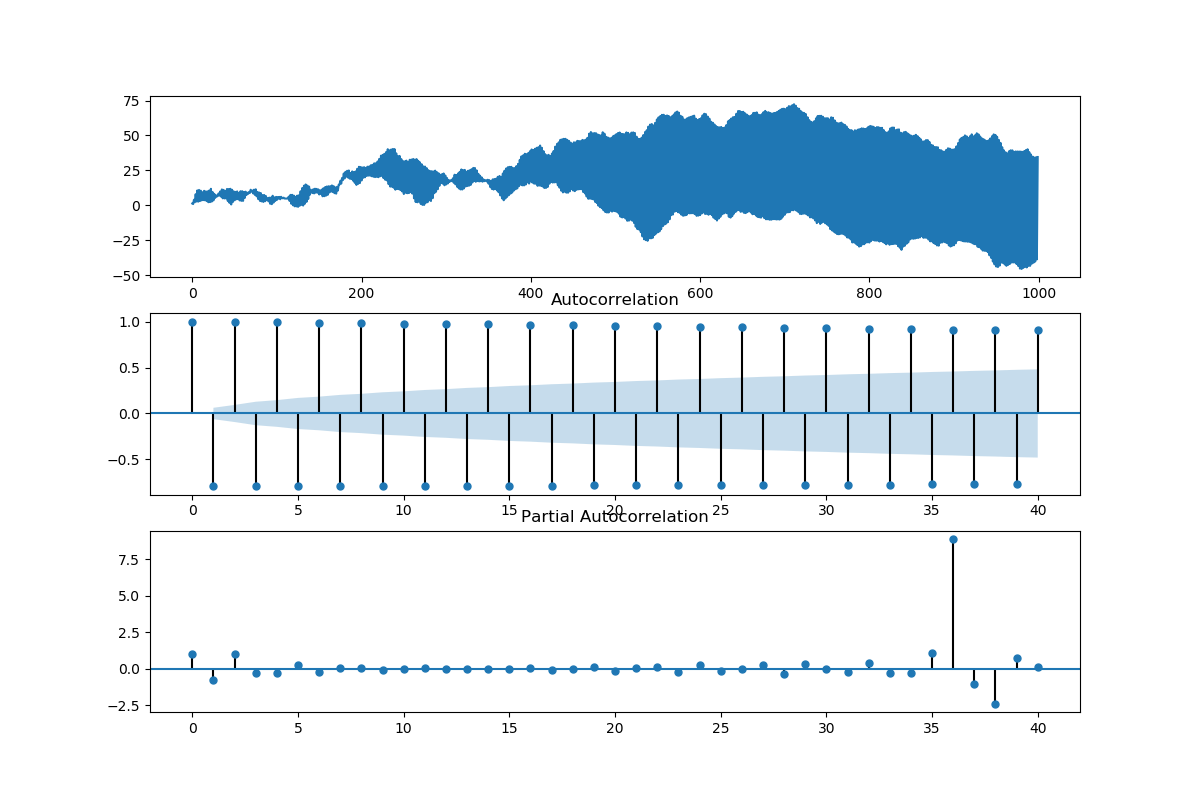
\includegraphics[scale=.5]{AR4NS.png}
\end{figure}
Graphiquement, on observe la non stationnarité des données et cela est vérifié par le test Dicker-Fuller augmenté : ADF : -1.4735 alors que les valeurs critiques sont 1\% : -3.437 5\%: -2.864 et 10\%: -2.568. On accepte l'hypothèse $H_0$ de non stationnarité.

\subsubsection{Processus mutlidimensionnel : VAR(p)}
\begin{Def}
Un processus vectoriel $\Xt$ de dimension (n,1) admet une représentation VAR d'ordre p, notée VAR(p) si~:
$$
X_t = c - \Phi_1X_{t-1}-\Phi_2X_{t-2}-...- \Phi_pX_{t-p}+\epsilon_t
$$
ou de façon équivalent~:
$$
\Phi(L)X_t = c+\epsilon_t
$$
où $c$ désigne un vecteur constant de dimension (n,1), $\Phi(L)=\sum_i\Phi_iL^i$. Le vecteur des innovation $\epsilon_t$ est i.i.d. centrée et de matrice covariance définie positive.
\end{Def}
Ainsi pour un vecteur de dimension (n,1) qui suit un processu VAR(p), on aura pour tout $j$~:
\begin{align*}
x_{j,t}=&c_1+\Phi_{j,1}^1x_{1,t-1}+\Phi_{j,2}^1x_{2,t-1}+....+\Phi_{j,n}^1x_{n,t-1}\\
& \Phi_{j,1}^2x_{1,t-2}+\Phi_{j,2}^2x_{2,t-2}+....+\Phi_{j,n}^2x_{n,t-2}\\
&+...+\\
& \Phi_{j,1}^px_{1,t-p}+\Phi_{j,2}^1x_{2,t-p}+....+\Phi_{j,n}^px_{n,t-p}
\end{align*}
Comme pour les processus AR(p) un processus VAR(p) sera stationnaire si et seulement si toutes racines du déterminant polynôme de retard $\Phi(L)$ sont toutes supérieures à l'unité en module. Ce qui est équivalent au fait que toute les valeurs propres de la 'application linéaire $\Phi(L)$ sont toutes inférieur à l'unité en module. Une conséquence du théorème de Wold (\ref{Wold}) est que tout processus VAR(p) stationnaire peut s'écrire sous la forme d'un processus VMA($\infty$). On peut également écrire le polynome $\Psi$ de la moyenne mobile à l'aide du polynome $\Phi$.
\begin{pro}
Le polynôme matriciel $\Psi(L)=\sum_i \psi_iL^i$ associé à la représentation VMA($\infty$) d'un processus VAR(p) stationnaire $\Phi(L)X_t = c + \epsilon_t$, satisfait la relation de récurrence suivante~:
\begin{align*}
\psi_0&=I_n\\
\psi_s &= \Phi_1\psi_{s-1}+\Phi_2\psi_{s-2}+...+\Phi_p\psi_{s-p},\forall s\geq 1\\
\psi_s&=0, \forall s <0.
\end{align*}
\end{pro}


Un propriété intéressante pour les processus VAR(p) stationnaire est qu'ils peuvent être transformé en un processus VAR(1) d'espérance nulle.
\begin{pro}
Tout processus vectoriel stationnaire $\Xt$ satisfaisant une représentation VAR(p) peut être transformé en un processus $\tilde{X}_t$ satisfaisant une représentation VAR(1) d'espérance nulle.
\end{pro}
\textit{preuve : }
\newline
On a pour tout $t$~:~$\Phi(L)X_t = c + \epsilon_t$ avec $\Phi(L)$ une matrice carrée de taille n. Comme $X_t$ est stationnaire, on a~:
$$
\E{X_t}=\Phi(L)^{-1}\E{c+\epsilon_t}=\Phi^{-1}(L)c=\mu
$$
On a donc~:
\begin{align*}
\Phi(L)(X_t-\mu) & = \epsilon_t\\
(X_t-\mu) & = \Phi_1(X_{t-1}-\mu)+...+\Phi_p(X_{t-p}-\mu)+\epsilon_t
\end{align*}
On pose~:
$$
\tilde{X}_t = \left(
\begin{array}{c}
X_t-\mu \\
X_{t-1}-\mu \\
X_{t-2}-\mu \\
...\\
X_{t-p+1}-\mu 
\end{array}
\right)
\quad
v_t = \left(
\begin{array}{c}
\epsilon_t \\
0_{(n,1)} \\
0_{(n,1)} \\
...\\
0_{(n,1)} 
\end{array}
\right)
$$
et 
$$
A = \left(
\begin{array}{ccccc}
\Phi_1 & \Phi_2 & ... & \Phi_{p-1} & \Phi_p \\
I_n & 0_{(n,n)} & ... & 0_{(n,n)} & 0_{(n,n)} \\
0_{(n,n)}& I_n & ... & 0_{(n,n)} & 0_{(n,n)} \\
...\\
0_{(n,n)}& 0_{(n,n)} & ... &  I_n& 0_{(n,n)} 
\end{array}
\right)
$$
il en résulte que $\tilde{X}_t$ est un processus VAR(1) qui s'écrit~:~$\tilde{X}_t = A\tilde{X_{t-1}}+v_t$, avec A une matrice carrée de taille np.
\subsubsection*{Exemple}
On considère le processus bi-varié $Y_t$~:
\begin{align*}
y_{1,t}&=3+ .2y_{1,t-2}+.7y_{2,t-1}-.4y_{1,t-2}-.6y_{2,t-2}+\epsilon_{1,t}\\
y_{2,t}&=1+ .3y_{1,t-2}+.4y_{2,t-1}-.1y_{1,t-2}-.8y_{2,t-2}+\epsilon_{2,t}
\end{align*}
le processus $Y_t$ sous forme matricielle~:
$$
\Phi(L)Y_t = c +\epsilon_t =
 \left(
\begin{array}{c}
3\\
1
\end{array}
\right)+
\left(
\begin{array}{c}
\epsilon_{1,t}\\
\epsilon_{2,t}
\end{array}
\right)
$$
avec 
\begin{align*}
\Phi(L)&=\Phi_0+\Phi_1L+\phi_2L^2\\
&=\left(
\begin{array}{cc}
1 & 0\\
0 & 1
\end{array}
\right) + 
\left(
\begin{array}{cc}
-.2 & -.7\\
-.3 & -.4
\end{array}
\right)L +
\left(
\begin{array}{cc}
.4 & .6\\
.1 & .8
\end{array}
\right)L^2 \\
&= \left( \begin{array}{cc}
1-.2L+.4L^2 & -.7L+.6L^2\\
-.3L+.1L^2 & 1-.4L+.8L^2\\
\end{array}
\right)
\end{align*}
Déterminons $\E{Y_t}$~:
$$
\E{Y_t} = \Phi(1)^{-1}c=\left(
\begin{array}{c}
2.59\\
1.8
\end{array}
\right)=\mu
$$
on pose alors~:
$$
\tilde{Y}_t = \left(
\begin{array}{c}
Y_t-\mu\\
Y_{t-1}-\mu
\end{array}
\right)=
\left(
\begin{array}{c}
y_{1,t}-2.59\\
y_{2,t}-1.8\\
y_{1,t-1}-2.59\\
y_{2,t-1}-1.8\\
\end{array}
\right)\quad \textrm{et}\quad v_t=\left(\begin{array}{c}
\epsilon_{1,t}\\
\epsilon_{2,t}\\
0\\
0
\end{array}\right)
$$
et
$$
A=\left(
\begin{array}{cccc}
-.2 & -.7 & .4 & .6\\
-.3 & -.4 & .1 & .8\\
1 & 0 & 0 & 0\\
0 & 1 & 0 & 0
\end{array}
\right)
$$
on obtient alors~:~$\tilde{Y}_t=A\tilde{Y}_{t-1}+v_t$
\subsection{processus ARMA}
\begin{Def}
Un processus $X_t$ d'ordre 2 (espérance $\mu$)est un processus ARMA(p,q), si et seulement si il est stationnaire et si pour $t$ il vérifie~:
$$
\phi(L)(X_t-\mu) = \theta(L)\epsilon_t
$$
avec $\epsilon_t$ est un bruit blanc de variance $\sigma^2$, $L$ le polynome de retard et~:
\begin{align*}
\phi(z)&=1-\phi_1z-...-\phi_pz^p\\
\theta(z)&=1+\theta_1z+...+\theta_qz^q
\end{align*}
\end{Def}
La fonction d'autocovariance des processus ARMA(p,q) suit la relation de récurrence~:
$$
\gamma_k=\phi_1\gamma_{k-1}+...+\phi_p\gamma_{k-p}\,,\forall k>q
$$
Il s'agit de la même relation de récurrence qu'un processus AR(p) (équations de Yule-Walker). On n'a pas la relation pour $k\leq q$. On obtient la même relation pour l'autocorellation. L'auto-corellation partielle d'un processus à le même comportement que pour les processus MA. L'écriture des processus ARMA va dépendre des racines des polynomes de retard correspondant au composant AR et MA
\begin{pro}
Soit $X_t$ un processus ARMA(p,q)~:~$\phi(L)X_t=\mu+\theta(L)\epsilon_t$, alors~:
\begin{itemize}
\item[i)] Si le polynôme $\phi$ ne s'annule pas sur le cercle unité alors $X_t$ est un processus linéaire
\item[ii)]Si le polynôme $\phi$ ne s'annule pas sur le disque unité alors $X_t$ admet une représentation causale
\item[iii)]Si le polynome $\theta$ ne s'annule pas sur le disque unité alors $X_t$ admet une représentation inversible
\end{itemize}
\end{pro}
En résumé~:
\begin{center}
\begin{tabular}{|c|c|c|c|}
\hline
Modèles & MA(q) & AR(p) & ARMA(p,q)\\
\hline
auto-correlation & $\rho(h)=0, \forall h>q$ &  $\rho(h)\rightarrow 0$ & $\rho(h)\rightarrow 0$ \\
\hline
auto-correlation partielle & $r(h)\rightarrow 0$ & $r(h)=0, \forall h>p$ &$r(h)\rightarrow 0$  \\
\hline
\end{tabular}
\end{center}
\subsection{ARIMA modèles}
Les problèmes ARMA sont utilisés pour des processus stationnaires. Lorsque les processus ne sont plus stationnaires on doit utiliser d'autre processus. Parmi ceux là il y a les processus ARIMA. Les processus ARIMA sont des processus non stationnaire mais qui deviennent stationnaire en transformant la série par différence finie.
\begin{Def}
Un processus $X_t$ admet une représentation ARIMA(p,q) s'il satisfait~:
$$
\Phi(L)(1-L)^dX_t=\theta(L)\epsilon_t
$$
avec $\epsilon_t$ un bruit blanc de variance $\sigma_t^2$. La représentation est minimale lorsque les polynomes $\Phi(L)$ et $\theta(L)$ non pas de racine commune.
\end{Def}
Une des propriété des processus ARIMA(p,d,q) est que le processus $(1-L)^dX_t$ est un processus stationnaire ARMA(p,q). On utilise la différence finie pour rendre stationnaire un processus non stationnaire.
\subsection{ARCH modèles}
Un des problèmes des modèles stationnaires est que la volatilité est constante dans le temps, pour certain types de données cela n'est pas le cas. Par exemple pour des données financières on observe des clusters de volatilité, i.e. une hausse est souvent suivi d'une hausse encore plus importante. Cela signifie que la série temporelle est corrélé en temps. Campbell, Lo and Mackinglay \cite{NonLinDef} ont défini différentes notions de non linéarité~:
\begin{Def}\label{nonlin}
\begin{itemize}
\item[i)] série temporelle linéaire~:~les chocs sont non corrélés mais nécessairement indépendant et identiquement distribué.\\
\item[ii)] série temporelle non linéaire~:~ les chocs sont supposés i.i.d, mais il y a des fonctions non linéaire associées à la série temporelle et aux chocs.
$$
X_t= g(\epsilon_{t-1},\epsilon_{t-2},...)+\epsilon_th(\epsilon_{t-1},\epsilon_{t-2},...)
$$
ainsi l'espérance de $X_t$ est donnée par g et la variance conditionnelle est donnée par $h^2$
\end{itemize}
\end{Def}
Ainsi on controle la variance conditionnelle via la fonction $h$. Les processus ARCH sont des processus non linéaires en variance conditionelle, d'espérance nulle et de variance constante. Ce type de comportement n'est pas possible pour des processus stationnaire. En effet d'après le théorème de Wold (\ref{Wold}) un processus stationnaire d'espérance nulle va s'écrire comme la somme infinie de bruit blanc~:
$$
X_t = \sum_{i\geq 0}\psi_i\epsilon_{t-i}
$$
avec $\psi_0=1$. Il en résulte que la variance est constante et que l'espérance conditionnelle s'écrit~: 
$$
\E{X_t|\epsilon_{t-1},\epsilon_{t-2},...}=\sum_{i\geq 1}\psi_i \epsilon_{t-i}
$$
Ainsi la variance conditionnelle d'un processus stationnaire est~:
\begin{align*}
\mathbb{V}\left(X_t|\epsilon_{t-1},\epsilon_{t-2},...\right)&= \E{\left(X_t-\E{X_t|\epsilon_{t-1},\epsilon_{t-2},...}\right)^2} \\
&= \E{\left(X_t-\E{X_t|\epsilon_{t-1},\epsilon_{t-2},...}\right)^2|\epsilon_{t-1},\epsilon_{t-2},...}\\
&= \E{\epsilon_t^2}\\
&= \sigma^2
\end{align*}
On obtient une variance conditionnelle qui est constante ce qui ne permet pas de modéliser les variances conditionnelles non linéaires. Afin de pouvoir le faire Engle \cite{archEngle} a défini les processus ARCH
\begin{Def}\label{archDef}
Un processus $z_t$ est un processus de ARCH(q), si l'on peut l'écrire sous la forme~:
\begin{align*}
z_t &= \epsilon_t\sigma_t\\
\sigma_t^2 &= \omega + \sum_{i=1}^q \alpha_i \epsilon_{t-i}^2\,,
\end{align*}
avec $\epsilon_t$ un bruit blanc fort de variance $1$ et $\omega,\alpha_1,\alpha_2,...,\alpha_q\geq 0$. 
\end{Def}
Dans le cas où le bruit blanc est un bruit blanc gaussien alors  la distribution conditionnelle de $z_t$ suit une loi normale~:
$$
z_t|z_{t-q},...,z_0\sim \mathcal{N}\left(0,\sigma_t^2\right)
$$
On peut vérifier que ce modèle à les propriétés souhaitées~:
\begin{align*}
\E{z_t|z_{t-1},...,z_0}&=\E{\epsilon_t\sigma_t|z_{t-1},...,z_0}\\
&=\E{\epsilon_t}\E{\sigma_t|z_{t-1},...,z_0}\\
&= 0\\
V(z_t|z_{t-1},...,z_0)&=\E{z_t^2|z_{t-1},...,z_0)}\\
&=\E{\sigma_t^2\epsilon_t^2|z_{t-1},...,z_0)}\\
&=\E{\sigma_t^2|z_{t-1},...,z_0)}\\
&= \sigma_t^2
\end{align*}
Si le processus admet des moments d'ordre 4, on en déduit tel que $\E{z_t^2}=\sigma^2<\infty$ et $\E{z_t^4}=c<\infty$, on en déduit pour un processus ARCH(q)~:
\begin{align*}
\E{z_t^2} &= \frac{\omega}{1-\alpha_1-...-\alpha_q},\textrm{ avec }\sum_{i=1}^q\alpha_i<1\\
\E{z_t^4}&\geq 3\E{\epsilon_t^2}^2
\end{align*}
Les processus ARCH(q) sont des processus dit \textit{fat tail}. C'est souvent le cas pour des données financières.
\subsection{GARCH modèles}
\begin{Def}\label{GARCHDef}
Un processus $z_t$ est un processus GARCH(p,q), si~:
\begin{align*}
z_t&=\epsilon_t\sigma_t,\textrm{ avec }\epsilon_t \textrm{ un bruit blanc fort de variance 1}\\
\sigma_t^2 &= \omega  +\sum_{i=1}^p\alpha_i z_{t-1}^2+\sum_{j=1}^q\beta_j\sigma_{t-j}^2
\end{align*}
\end{Def}
Les processus de type GARCH vérifient les propriétés suivantes~: l'espérance est nulle, autocorellation est nulle pour tout lag h>0.
\begin{align*}
\E{z_t}&= \E{\sigma_t\epsilon_t}=\E{\E{\sigma\epsilon_t|z_{t-1},...}}=\E{\sigma_t\E{\epsilon_t|z_{t-1},...}}=\E{\sigma_t\E{\epsilon_t}}=0\\
\E{z_tz_{t+h}}&=\E{\sigma_t\epsilon_t\sigma_{t+h}\epsilon_{t+h}}=\E{\E{\sigma_t\epsilon_t\sigma_{t+h}\epsilon_{t+h}|z_{t+h-1},...}}=0
\end{align*}
On remarque aussi le processus $z_t^2$ est un processus ARMA(p,q)~:
$$
z_t^2= \sigma_k^2+(y_k^2-\sigma_k^2)=\sigma_k^2+\sigma_k^2(\epsilon_k^2-1)
$$
en posant $\tilde{\epsilon_t}=\sigma_k^2(\epsilon_k^2-1)$ on a~:
\begin{align*}
z_t^2&= \omega  +\sum_{i=1}^p\alpha_i z_{t-1}^2+\sum_{j=1}^q\beta_j\sigma_{t-j}^2 + \tilde{\epsilon_t}\\
&=\omega  +\sum_{i=1}^p\alpha_i z_{t-1}^2+\sum_{j=1}^q\beta_j\sigma_{t-j}^2 + \tilde{\epsilon_t}\\
&=\omega  +\sum_{i=1}^p\alpha_i z_{t-1}^2+\sum_{j=1}^q\beta_j( z^2_{t_j}-\tilde{\epsilon}_{t-j} )+ \tilde{\epsilon_t}\\
&=\omega  +\sum_{i=1}^{max(p,q)}\left(\alpha_i+\beta_i\right) z_{t-1}^2-\sum_{j=1}^q\beta_j\tilde{\epsilon}_{t-j}+ \tilde{\epsilon_t}\\
\end{align*}
On peut alors utiliser les résultats des processus ARMA afin de décrire le processu $z_t^2$ et donc d'obtenir la variance du processus $z_t$. Sous la condition de stationnarité, on a~:
$$
V(z_t)=\E{y_t^2}=\frac{\omega}{1-\sum_{i=1}^{max(p,q)}\alpha_i+\beta_i}
$$
Comme pour les processus ARCH, les processus GARCH sont des processus de type \textit{fat tails}. Il existe des extensions des processus GARCH tels que les processus EGARCH \textit{exponential GARCH} ou IGARCH \textit{integrated GARCH}.
\subsection{Estimation des paramètres}
\subsubsection{modèle ARMA}
L'estimation des paramètres d'un modèle ARMA(p,q) lorsque les ordres p et q sont supposés connus peut se réaliser par différentes méthodes dans le domaine temporel~:
\begin{itemize}
\item Moindres carrés Ordinaires pour les modèles sans composante MA. Dans ce cas on utilise les équations de Yule Walker. En remplacant les autocorrélations théoriques par leurs estimateurs, on peut retrouver les estimateurs des MCO des parmètres du modèle par la résolution des équations de Yule Walker.\\
\item maximum de vraisemblance
\end{itemize}
Je vais détailler ici l'approche par maximum de vraisemblance, elle sera utilisée dans les tests pratiques. Un rappel sur l'estimateur du maximum de vraisemblance se trouve en annexe.

Afin de pour voir appliquer l'estimation par maximum de vraisemblance sur les modèles ARMA, on doit décrire la vraisemblance du modèle. Pour cela on va supposer que le bruit blanc décrivant le processus ARMA est gaussien de variance $\sigma^2$. Ainsi pour tout processus ARMA(p,q)~:~$\Phi(L)x_t = c+ \Theta(L)\epsilon_t$, avec $\theta_0=\phi_0=1$,  la vraisemblance associé au vecteur de réalisation $(x_1,..,x_T)$ s'écrit alors~:
\begin{equation}\label{MLEARMA}
(2\pi\sigma^2)^{-\frac{T}{2}}det\left[\right]^{-\frac{1}{2}}exp\left(-\frac{1}{2\sigma^2}x'\left[(\theta_i,\phi_i)]\right]^{-1}x\right)
\end{equation}

Les paramètres $\hat{\phi}$ et $\hat{\theta}$ sont ceux qui maximise cette fonction de vraisemblance, comme la fonction est $C^2$ on peut utiliser les dérivées partielles à l'ordre 2 pour les déterminer. Une fois ces paramètres trouver on va devoir appliquer plusieurs tests afin de simplifier la forme obtenue. Un premier test est le \textit{test de redondance} dont le but est de vérifier si les composantes AR et MA de l'ARMA non pas de racines communes. Si tel est le cas on peut alors se ramener à une représentation minimal excluant ces racines. En effet si le processus ARMA(p,q) $x_t$ est tel que~:
$$
\Phi(L)x_t=\Theta(L)\epsilon_t
$$
et que les polynomes $\Theta(L)$ et $\Phi(L)$ ont une racine commune $\lambda$ alors on a~:
\begin{align*}
\Phi(L)&=(1-\frac{L}{\lambda})\tilde{\Phi}(L)\\
\Theta(L)&=(1-\frac{L}{\lambda})\tilde{\Theta}(L)\\
\end{align*}
avec $\tilde{\Phi(L)}$ (resp. $\tilde{\Theta(L)}$) un polynome de degré p-1 (resp. q-1). En divisant les polynomes par ce facteur commun, on obtient une nouvelle représentation de $x_t$~:
$$
\tilde{\Phi}(L)x_t=\tilde{\Theta}(L)\epsilon_t
$$
en faisant de même pour toutes les racines communes ont obtient la représentation minimale du processus. 

Afin de vérifier que les paramètres obtenus sont significativement différent de 0, on applique un test de significativité des coefficents obtenues. Pour cela on utilise le résultat suivant 
\begin{theorem}
L'estimateur du maximum de vraisemblance du vecteur des paramètres du modèle ARMA(p,q), noté $\hat{\Delta}=\left(\hat{\phi}_1,...,\hat{\phi}_p,\hat{\theta}_1,...,\hat{\theta}_q\right)$ est asymptotiquement distribué suivant une loi normale de moyenne $\Delta$ et de matrice de covariance $\mathbb{E}\left(\hat{\Delta}\hat{\Delta}'\right)=\mathcal{F}^{-1}$, avec $\mathcal{F}$ la matrice d'information de Fischer~:
$$
\mathcal{F}=-\mathbb{E}\left(\frac{\partial^2L(x,\Delta)}{\partial\delta_i\delta_j}\right)
$$
avec $\delta_i,\delta_j\in \Delta$.
\end{theorem}
On peut donc appliquer à ces estimateurs les méthodes d'inférence tradionnelle car assymptotiquement distribué selon une loi normale. Ainsi si l'on montre qu'un ou plusieurs paramètres ne sont pas significativement différents de 0, on estime à nouveau le modèle en excluant les variables correspondantes.
\subsubsection{processus ARIMA}
Pour les processus ARIMA, on va se ramener par différences premieres à un processus ARMA, on va estimer les paramètres sur les données ainsi filtrés. On reconstruit ensuite par inversion du filtre sur la série initiale.
\subsubsection{méthodologie de Box Jenkins}
Une fois le modèle choisi on peut générer des échantillons suivant la diffusion du processus choisi. Pour cela on peut par example utiliser la librairie statsmodels en python. Mais le problème inverse est plus complexe. Comment à partir de données peut-on trouver le modèle qui estime au mieux ses données. La méthodologie de Box Jenkins propose une façon d'estimer les paramètres du modèle ARIMA.


La méthode de Box-Jenkins \cite{BoxJenkins} ne présuppose d'aucun pattern dans les données. Il utilise tros étapes itératives~:
\begin{itemize}
\item[i)] identification du modele
\item[ii)] estimation des paramètres
\item[iii)] verification
\end{itemize}
Cette méthode itérative permet de déterminer parmi les modeles ARIMA ceux qui correspondent aux mieux (selon un critère donné : AIC, BIC, HQIC ...) aux données.
Une étape crucial dans la selection du modele est l'estimation des paramètre et le choix de la métrique de classification. Un critère pour le choix des paramètres va être fourni par l'ACF et le PACF. En effet, on peut calculer l'ACF et le PACF sur l'échantillon fournit et à l'aide des résultats théorique sur les procesus ARMA et ARIMA en déduire un intevalle de valeur possible pour les paramètres p,q et d. Une fois la grille fournit de test fournit on calcule les critères AIC ou BIC pour chacun des paramètre. Le meilleur modèle sera celui qui minimise les critères. Les critères AIC et BIC sont définis de la manière suivante~:
\begin{align*}
AIC(p)&=n\ln\left({\frac{\hat{\sigma}_e^2}{n}}\right)+2p\\
BIC(p)&=n\ln\left({\frac{\hat{\sigma}_e^2}{n}}\right)+p+p\ln(n)
\end{align*}
avec n le nombre d'observations utilisé pour estimer le modele, p est le nombre de paramètres du modèle et $\hat{sigma}_e^2$ est la somme des résidus (SSR). L'intéret des critères AIC et BIC et de tenir compte l'erreur quadratique (SSR) mais aussi de la complexity du modèle. Ainsi le modele qui minimise les critères ACI ou BIC sera celui qui fournit une bonne approximation relativement à la complexité du modele.
\section{Réseaux de neurones}
\subsection{RNN}
Les réseaux récurrents – RNNs dans la suite – permettent de traiter des données séquentielles, une suite d’entrées $x_0, . . . ,x_m$. En effet au temps $t$ ils calculent leur sortie en fonction de l’entrée $x_t$ mais aussi de l’état de la couche cachée au temps précédent. Ainsi ils font évoluer un état interne qui fait office de mémoire à court terme et qui permet de prendre en compte les dépendances temporelles que manifestent les entrées. Les RNNs les plus simples se décrivent de la manière suivante~:
\begin{Def}\label{VanillaRNN}
Soient $n,p,k\in \N$, $x_0,...,x_m$ une suite d'entrée, $W\in \R^{k,n}$, $W_h\in \R^{k,k}$, $O\in \R^{p,k}$ et $h_{-1}\in\R^k$ alors la dynamique du RNN simple (ou Vanilla RNN) associé est décrite par~:
\begin{eqnarray}
h_t &=& \sigma(Wx_t+W_gh_{t-1})\\
y_t&=&Oh_t
\end{eqnarray}
avec $h_t$ l'état de la couche cachée et $y_t$ l'état de la couche de sortie. Dans la suite on utilisera indifféremment RNN pour \textit{Vanilla RNN}.
\end{Def}
On peut visualiser ces RNNs sous forme de graphe~:
\begin{center}
\def\layersep{2.5cm}
\begin{tikzpicture}[shorten >=1pt,->,draw=black!50, node distance=\layersep]
    \tikzstyle{every pin edge}=[<-,shorten <=1pt]
    \tikzstyle{neuron}=[circle,fill=black!25,minimum size=17pt,inner sep=0pt]
    \tikzstyle{input neuron}=[neuron, fill=green!50];
    \tikzstyle{output neuron}=[neuron, fill=red!50];
    \tikzstyle{hidden neuron}=[neuron, fill=blue!50];
    \tikzstyle{annot} = [text width=4em, text centered]

    % Draw the input layer nodes
    \foreach \name / \y in {1,...,4}
    % This is the same as writing \foreach \name / \y in {1/1,2/2,3/3,4/4}
        \node[input neuron, pin=left: $(x_t)_\y$] (I-\name) at (0,-\y) {};

    % Draw the hidden layer nodes
    \foreach \name / \y in {1,...,5}
        \path[yshift=0.5cm]
            node[hidden neuron] (H1-\name) at (\layersep,-\y cm) {};
    
    % Draw the hidden layer nodes
    \foreach \name / \y in {1,...,5}
        \path[yshift=0.5cm]
            node[hidden neuron] (H2-\name) at (2*\layersep,-\y cm) {};

    % Draw the output layer node
    \node[output neuron,pin={[pin edge={->}]right:$y_t$}, right of=H2-3] (O) {};

    % Connect every node in the input layer with every node in the
    % hidden layer.
    \foreach \source in {1,...,4}
        \foreach \dest in {1,...,5}
            \path (I-\source) edge (H1-\dest);
	
	% Connect every node in the input layer with every node in the
    % hidden layer.
    \foreach \source in {1,...,5}
        \foreach \dest in {1,...,5}
            \path (H1-\source) edge (H2-\dest);	
	
    % Connect every node in the hidden layer with the output layer
    \foreach \source in {1,...,5}
        \path (H2-\source) edge (O);

    % Annotate the layers
    \node[annot,above of=H1-1, node distance=1cm] (hl) {Couche cachée à t-1};
    \node[annot,above of=H2-1, node distance=1cm] (h2) {Couche cachée à t};
    \node[annot,left of=hl] {Couche d'entrée};
    \node[annot,right of=h2] {Couche de sortie};
\end{tikzpicture}
\end{center}
Les RNNs forment un modèle très puissant, ils sont Turing complet et on peut implémenter n'importe quel algorithme avec cette architecture. Mais en pratique, il est difficile d'entrainer les RNNs à cause du \textit{vansihing or exploding gradient}. Lors de la descente du gradient temporelle BTT \textit{Backpropagation Through Time} le gradient s'anulle ou explose numériquement. C'est pour remédier à ce problème de \textit{vanishing gradient} que le modèle LSTM a été créé \cite{LSTM}
\subsection{LSTM}
\subsection{GRU}
\section{Annexe}
\subsection{Convergence}
Convergence $\mathcal{L}^2$~:
$$
X_n\rightarrow_{\mathcal{L^2}} X \Leftrightarrow  \lim_{n\rightarrow \infty}||X_n-X||_2=0
$$
On dit que $X_t$ convergent en loi vers $X$ si et seulement si pour toute fonction bornée $\phi$, on a~:~
$$
\lim_{n}\mathcal{E}(\phi(X_n))=\mathcal{E}\left(\phi(X)\right)
$$
\subsection{Inversibilité}
Pour un processus définit à partir de bruit blanc, on aimerait pouvoir exprimer ce processus en fonction du passé (observé) et pas seulement en fonction du bruit blanc non observé. C'est la question de l'inversibilité du processus. Cela veut donc dire qu'un processus est inversible si on peut le représenter comme une autorégression infinie $AR(\infty)$. Ainsi un processus AR(p) est toujours inversible et pour un processus MA(q) la condition d'inversibilité est similaire à la condition de stationnarité des processus AR~:
\begin{pro}
Un processus MA(q) défini par : $X_t=\Theta(L)\epsilon_t$, avec $\epsilon_t$ un bruit blanc et $\theta_0=1$, est inversible si les racines du polynome $ \Theta(L)$ sont, en module, strictement supérieures à 1
\end{pro}
\subsection{Densité spectrale}
Les coefficients d'autocovariance d'une série stationnaire correspondent aux coefficients de Fourier d'une mesure positive, appelée mesure spectrale du processus. Il est possible de montrer que cette mesure spectrale admet un densité, dite spectrale, par rapport à la mesure de Lebesgues sur $[-\pi,\pi]$ que nous noterons $f_X$.
\begin{Def}
Soit $\Xt$ un processus de fonction d'autocovariance $\gamma_X$ la densité spectrale $f_X$ de $\Xt$ s'écrit~:
$$
f_X(\omega) = \frac{1}{2\pi}\sum_{h\in\mathbb{Z}}\gamma_X(h)e^{-i\omega h}\,.
$$
\end{Def}
\begin{pro}
Si $f_X$ est la densité spectrale de $\Xt$ alors~:
$$
\gamma_X(h)=\int_{-\pi}^{\pi}f_X(\omega)e^{i\omega h}d\omega
$$
\end{pro}
Le principal outil d'analyse dont on dispose pour estimer empiriquement la densité spectrale théorique du processus est le périodogramme $I_T$, défini sur l'intervalle $[0,2\pi[$ par~:
$$
I_T(\lambda)=\frac{1}{2\pi T}\left|\sum_{t=1}^Te^{-i\lambda t}X_t\right|^2
$$

\subsubsection*{Exemple}
Par exemple pour un bruit blanc fort (\ref{BB}), on a~:
$$
\left\{
\begin{array}{cc}
\gamma(0)=\sigma^2&\\
\gamma(h)= 0,& \textrm{pour $h\not=0$} 
\end{array}
\right.
$$
ainsi la densité spectrale du bruit blanc fort s'écrit~:
$$
f_X(\omega) = \frac{\sigma^2}{2\pi}
$$





La densité spectrale peut être utilisée pour déterminer si un processus est un bruit blanc.
\begin{pro}
Si la densité spectrale d'une série $\Xt$ est constante alors ce processus est un bruit blanc fort.
\end{pro}
En effet~:
$$
\gamma_X(h)=\int_{-\pi}^{\pi}f_X(\omega)e^{i\omega h}d\omega = K\int_{-\pi}^{\pi}e^{i\omega h}d\omega
$$
et donc si $h=0$ alors $\gamma_X(h)=2\pi K$ et si $h\not=0$ alors $\gamma_X(h)=0$. Ceci caractérise un bruit blanc. La densité spectrale peut être utilisée pour décrire les dépendances entre les processus.
\begin{pro}
Si $\Xt$ est une moyenne mobile~:
$$
X_t = \sum_{k\in\mathbb{Z}}a_k\epsilon_{t-k}\,,
$$
où $\epsilon_t$ est un bruit blanc fort de variance $\sigma^2$ et tel que $\sum_{k\in\mathbb{Z}}|a_k| <+\infty$. Si on considère $Y_t = \sum_{j\in\mathbb{Z}}\beta_jX_{t-j}$, alors on a la relation suivante~:
$$
f_Y(\omega)=f_X(\omega)\left|\sum_{j\in\mathbb{Z}}\beta_je^{i\omega j}\right|^2
$$
\end{pro}
Par exemple si $Y_t=X_t-\phi X_{t-1}$ on a~:$f_Y(\omega)=f_X(\omega)\left|1-\phi e^{i\omega}\right|^2.$
\subsection{Estimateur empirique des moments}
Soit $(X_t)_{t\in\mathbb{Z}}$ un processus stationnaire, on cherche à estimer l'espérance, les fonction d'auto-covariance, d'auto-corrélation et d'auto-corrélation partielle. On a un échantillon de taille T. On prend comme estimateur~:
\begin{itemize}
\item moyenne empirique~:~$\hat{m}=\frac{1}{T}\sum_{t=1}^TX_t=\overline{X}_T$\\
\item auto-covariance empirique d'ordre h~:~$\hat{\gamma}(h)=\frac{1}{T-h}\sum_{t=h+1}^T(X_t-\overline{X}_T)(X_{t-h}-\overline{X}_T)$\\
\item auto-corrélation empirique d'ordre h~:~$\hat{\rho}(h)=\frac{\hat{\gamma}(h)}{\hat{\gamma}(0)}$.\\
\item l'auto-corrélation partielle est une régression empirique sur 1,$X_1$,...,$X-{t-h}$.
\end{itemize}
Pour estimer la fonction de densité spectrale on utilise la auto-covariance empirique et un terme d'ajustement (coefficient de Newey-West) afin diminuer le poids de $\hat{\gamma}(h)$ pour des h grand.


Si $X_t$ est un processus stationnaire alors d'après la loi des grands nombres tous les estimateurs empiriques présentés ci-dessus convergent.

\begin{pro}
Si $X_t=m+\sum_{j\geq 0}a_j\epsilon_{t-j}$ avec $\epsilon_t$ un bruit blanc de moment d'ordre 4 fini, alors tous ses estimateurs ont des lois jointes asymptotiquement gaussiennes~:
$$
\sqrt{T}\left(\hat{m}-m\right)\rightarrow \mathcal{N}(0,\sum_{h\in\mathcal{Z}}\gamma(h)
$$
convergence en loi
\end{pro}
\subsection{polynôme de retard}
\begin{Def}
L'opérateur de retard est défini sur la classe des processus stationnaires comme étant~: 
$$
L(X_t)=X_{t-1}
$$
\end{Def}
\begin{Def}
Soit $P$ un polynôme, $P(z)=\sum_{k=0}^{p}a_kz^k$ avec $a_k\in\mathbb{R}$, on lui associe le polynôme de retard $P(L)$ défini comme suit~:
$$
P(L)=\sum_{k=0}^pa_kL^k
$$
et 
$$
P(L)X_t=\sum_{k=0}^pa_kX_{t-k}
$$
\end{Def}
Un polynôme de retard P(L) est inversible s'il existe un polynôme de retard $Q(L)$ tel que $P(L)Q(L)=Id$. Dans $\mathbb{C}$, tout polynôme réel $P$ se décompose~:
$$
P(z)=\prod_{i=1}^p(z-z_i)=\prod_{i=1}^p(-z_i)\prod_{i=1}^p(1-\frac{z}{z_i})=\alpha\prod_{i=1}^p(1-\lambda_i z)
$$
avec $\lambda_i=\frac{1}{z_i}$.
Le polynôme est $(1-\lambda z)$ est inversible si seulement si ses racines sont de modules strictement inférieur à 1. Ceci équivalent à $|\lambda|>1$. On peut généraliser ce résultat à tout polynôme de degré p.
\begin{pro}
Soit $P(L) = \alpha\prod_{i=1}^p(1-\lambda_i L)$ un polynôme de retard, si pour tout i $|\lambda_i|<1$ alors $P(L)$ est inversible et :
$$
P^{-1}(L)= \sum_{k\geq 0}b_kL^k
$$
\end{pro}

\subsection{Chaine de Markov}
\begin{Def}
Le processus $\left\{X_t\right\}_{t\in\mathbb{N}}$ est une chaîne de Markov d'ordre p si et seulement si, pour tout $t$, on a l'égalité de distributions~:
$$
\mathcal{L}\left(X_t|X_{t-1},X_{t-2},X_{t-3},....\right) = \mathcal{L}\left(X_t|X_{t-1},...,X_{t-p}\right)
$$
\end{Def}
\begin{theorem}
Le processus $\left\{X_t\right\}_{t\in\mathbb{N}}$ est une chaine de markov d'ordre 1 si et seulement s'il existe une fonction $g$ mesurable et un processus $\epsilon_t$ tel que $X_t=g(X_{t-1},\epsilon_t)$ avec $\epsilon_t$ une suite de variable aléatoire indépendante et de même loi.
\end{theorem}
Un processus AR(1) est un processus markovien, de même toute marche aléatoire une processus markovien d'ordre 1.
\subsection{Estimateur du maximum de vraisemblance}
\begin{Def}\label{estimateur}
Soit $X$ une variable aléatoire de loi $P_{\theta}$. On note $f(x,\theta)$ la densité de $P_{\theta}$ et $f(x_1,...x_n,\theta)$ la densité empirique correspondante. On appelle vraisemblance du paramètre $\theta$ l'application $\Theta\rightarrow\mathbb{R}^+$ définie par~:
\begin{align*}
\Theta &\rightarrow \mathbb{R}^+\\
\theta &\mapsto L(x_1,...,x_n,\theta)=\prod_{i=1}^n f(x_i,\theta)
\end{align*}
\end{Def}
\begin{Def}\label{MLE}
Soit $L(x,\theta)$ la vraisemblance au point $\theta$, on appelle estimateur du maximum de vraisemblance pour $\theta$ la statistique $\hat{\theta}$ pour les observations $x_1,...,x_n$ telle que~:
$$
\forall \theta \, ,  L(x,\hat{\theta})\geq L(x,\theta)
$$
\end{Def}
Le principe de vraisemblance revient à déterminer la valeur du paramètre $\theta$, fonction des observations $x_1,...,x_n$, qui assure la plus grande porbabilité d'apparition de ces observations $(x_1,...,x_n)$.
\begin{corollary}
Lorsque l'on suppose que $X$ est à valeur dans un ensemble qui est indépendant de $\theta$ et que la fonction de vraisemblance $L$ est $C^2$ par rapport à $\theta$, alors l'estimateur du maximum de vraisemblance $\hat{\theta}$ est solution du système~:
\begin{eqnarray}
\left(\frac{\partial L(x,\theta)}{\partial \theta}\right)&=&0\\
\left(\frac{\partial^2 L(x,\theta)}{\partial \theta^2}\right)&<&0
\end{eqnarray}
\end{corollary}
Afin de déterminer la qualité d'une estimation il existe différentes métriques comme par exemple le coefficient de détermination. Le coefficient de détermination donne une information sur la part de la variance de la variable endogène (ici $x_t$) qui peut être expliquée par la modèle estimé.
\begin{Def}
Soit un processus $x_t$, on note $\hat{\epsilon}_t$ le résidu d'estimation du modèle. Les coefficients de détermination $R^2$ et $\overline{R}^2$ sont alors définis par~:

\begin{eqnarray}
R^2&=&1-\frac{\sum_{t=1}^T\hat{\epsilon}_t^2}{\sum_{t=1}^T\left(x_t-\overline{x}\right)^2}\\
\overline{R}^2&=&1-\frac{T-1}{T-n}\frac{\sum_{t=1}^T\hat{\epsilon}_t^2}{\sum_{t=1}^T\left(x_t-\overline{x}\right)}
\end{eqnarray}
avec $n$ le nombre de paramètres à estimer, par exemple pour un modèle ARMA(p,q) on a $n=p+q$.
\end{Def}
Un ajustement parfait est obtenue pour $R^2=1$.
\subsection{Test statistiques}
\subsubsection{Test de bruit blanc}
Lorsque le processus est bien estimé, les résidus entre les valeurs observées et les valeurs estimées par le modèle doivent se conporter comme un bruit blanc. On notera par la suite $\hat{\epsilon}_t$ le résidu d'estimation du modèle. Pour un modèle ARMA ou ARIMA on suppose que le processus $\epsilon_t$ est un bruit blanc gaussien centré de variance $\sigma^2$, ainsi par le théorème centrale limite on doit avoir :
$$
\frac{\overline{\epsilon}_t\sqrt{T}}{\sigma^2}\rightarrow_{T\rightarrow\infty}\mathcal{N}(0,1)
$$
avec $\overline{\epsilon}_t$ la moyenne des résidus. on peut donc test la nullité de la moyenne des résidus en construisant un intervalle de confiance au seuil adequat.

On peut aussi vérifier l'autocorellation des résidus via les tests de Durbin-Watson, test de Box et Pierce ou de Ljung-Box par exemple. Si les résidus obéissent à un bruit blanc il ne doit pas y avoir d'autocorrélation dans la série.

Afin de vérifier si les résidus sont des processus gaussien on peut utiliser des tests de normalité tels que le test de Jarque et Bera.
\subsection{Critère de convergence}
Pour les modèles AR, MA, ARMA et ARIMA par exemple plutot que d'utiliser les métriques classiques telles que MAE, RMSE par exemple on va utiliser les critères tenant compte de la complexité du modèle~:
\begin{itemize}
\item[$\bullet$] Critère de Akaike (AIC) : le meilleur des modèles ARMA(p,q) est le modèle qui minimise~: $AIC(p,q)=T\log\left(\sigma_{\hat{\epsilon}_t}^2\right)+2(p+q)$\\
\item[$\bullet$] Critère d'information Bayésien (BIC) : ce critère présente l'avantage de plus pénaliser les modèles où les paramètres sont en surnombre comparativement à l'AIC~: $$BIC(p,q)=T\log\left(\sigma_{\hat{\epsilon}_t}^2\right)-(n-p-q)\log\left(1-\frac{p+q}{T}\right)+(p+q)\log(T)+\log\left((p+q)^{-1}\left(\frac{\sigma_x^2}{\sigma_{\hat{\epsilon}^2}-1}\right)\right)$$
\item[$\bullet$] le critère de Schwarz~:~$SC(p,q)=T\log\left(\sigma_{\hat{\epsilon}}^2\right)+(p+q)\log(T)$\\
\item[$\bullet$] le critère de Hannan-Quin~:~$HQ(p,q)=\log(\sigma_{\hat{\epsilon}}^2)+(p+q)c\log\left(\frac{log(T)}{T}\right)$ avec $c$ une constante à spécifier.
\end{itemize}
\bibliographystyle{amsplain}
%\bibliography{C:/Users/jerpetit/Desktop/master/TRIED/memoireM2/biblio}
\bibliography{C:/Users/jerom/PycharmProjects/memoireM2/biblio}
\end{document}
